\documentclass[a4paper, 12pt]{report}
\usepackage[spanish]{babel}
\usepackage[utf8]{inputenc}
\usepackage{textcomp}
\usepackage{booktabs}
\usepackage{amssymb}
\usepackage{bussproofs}
\usepackage{algpseudocode}

\usepackage{fancyhdr}
\usepackage{graphicx}
\usepackage{amsmath}

\pagestyle{fancy}
\lhead{Almeida, Arteaga \& Eugenio}
\chead{Tarea 1}
\rhead{\today}

\begin{document}
\begin{titlepage}
    \centering
    {\scshape\Huge Universidad Nacional Autónoma de México \par}
    \vspace{1.5cm}
    {\scshape\huge Análisis de Algoritmos\par}
    \vspace{1.25cm}
    {\huge\bfseries Tarea 1\par}
    \vspace{1.5cm}
    {\Large\textsc Almeida Rodríguez Jerónimo\par}
    \vspace{.1cm}
    {\large\texttt{ jalrod@ciencias.unam.mx}\par}
    \vspace{0.5cm}
    {\Large\textsc Arteaga Vázquez Alan Ernesto\par}
    \vspace{.1cm}
    {\large\texttt{alanarteagav@ciencias.unam.mx}\par}
    \vspace{0.5cm}
    {\Large\textsc Eugenio Aceves Narciso Isaac \par}
    \vspace{.1cm}
    {\large\texttt{isaacn97@ciencias.unam.mx}\par}
    \vspace{2cm}
    \vfill
    \begin{figure}[hb!]
        
\includegraphics[width=.3\textwidth]
            {../logos/escudo_f-ciencias.png}\hfill
        
\includegraphics[width=.3\textwidth]
            {../logos/Escudo_UNAM.png}\hfill
    \end{figure}
\end{titlepage}
\begin{enumerate}
\item[1)]{
\begin{enumerate}
    \item[1)]{
        Propuesta de algoritmo:\\
        \begin{algorithmic}[1]
        \Procedure{POSITIVOS}{$A[\ ]$}\Comment{Recibe un arreglo con $n\geq 0$ enteros}
        \State $is\_positive\gets True$
        \State $array\_index\gets 0$
        \If{$len(A[]) == 0$}
            \State \textbf{return} True\Comment{Por vacuidad devuelve True}
        \EndIf
        \While{$array\_index < len(A[\ ])$}
            \State $is\_positive\ \&=\ A[array\_index] \geq 0$
            \State $array\_index\ += 1$
        \EndWhile\label{euclidendwhile}
        \State \textbf{return} $is\_positive$
        \EndProcedure
    \end{algorithmic}
    }
    \item[2)]{\bf Argumento de correctud:\\}
    Mostramos por invariante que el ciclo interno al
    algoritmo POSITIVOS es correcto:\\

    Invariante: Después de recorrer un índice en el arreglo, la variable
    $is\_positive$ es TRUE si no se ha encontrado un número negativo, de lo
    contrario, se almacena la variable FALSE.
    \begin{itemize}
        \item {\it Inicialización:}
            Antes del ciclo, se inicializa la variable $is\_positive$ a la
            constante TRUE pues al no haber recorrido el arreglo (línea 2), por
            vacuidad
            no se puede hallar ningún número negativo, por lo cual, se cumple
            la propiedad.
        \item {\it Mantenimiento:}
            Suponemos que la propiedad se cumple en una iteración previa del
            ciclo, queremos mostrar que se cumple después de una nueva
            iteración.\\
            Como la propiedad se cumple, en la variable $is\_positive$ se
            encuentra la constante TRUE si no se ha hallado ningún número
            negativo, FALSE en otro caso. Por la línea 8, se consulta el valor
            del número en el índice actual y se realiza una comparación de
            'mayor o igual' con el número cero. Si el número es positivo, la
            comparación resulta en un booleano TRUE, de lo contrario, resulta
            en un booleano FALSE. Consideremos ahora el valor booleano de la
            comparación, de acuerdo a la línea 8, se le aplica la operación
            booleana 'AND' al resultado de la comparación junto con el valor
            booleano almacenado en $is\_positive$. Se tienen ahora los
            siguientes casos:
            \begin{itemize}
                \item Si $is\_positive$ era TRUE, y el valor de la comparación
                    es TRUE, la operación $\&$ (AND) regresa TRUE lo cual se
                    asigna a
                    la variable $is\_positive$, manteniendo la
                    propiedad de que $is\_positive$ es TRUE al no haberse encontrado un número negativo.
                \item Si $is\_positive$ era TRUE, y el valor de la comparación
                    es FALSE, la operación $\&$ regresa FALSE lo cual se asigna a
                    la variable $is\_positive$, así, $is\_positive$ cumple
                    el invariante, al ser FALSE cuando se acaba de hallar un
                    número negativo.
                \item Si $is\_positive$ era FALSE, y el valor de la comparación
                    es FALSE, la operación $\&$ regresa FALSE lo cual se asigna
                    a
                    la variable $is\_positive$, así, $is\_positive$ cumple
                    el invariante, al ser FALSE cuando se acaba de hallar un
                    número negativo.
                \item Si $is\_positive$ era FALSE, y el valor de la comparación
                    es TRUE, la operación $\&$ regresa FALSE lo cual se asigna
                    a
                    la variable $is\_positive$, así, $is\_positive$ cumple
                    el invariante, al continuar siendo FALSE por haberse
                    hallado previamente un número negativo.
            \end{itemize}
            Al fin del ciclo, se incrementa $array\_index$ en una unidad, lo
            cual permite continuar con la iteración.
        \item {\it Mantenimiento:}
            La cláusula del ciclo while establece que este se rompe cuando la
            variable $array\_index$ es igual a la longitud del arreglo, por lo
            cual, se ha recorrido exitosamente la totalidad del mismo. Al
            haber terminado de recorrer el arreglo, la variable $is\_positive$
            mantiene el valor requerido al no modificarse una vez recorrida la
            totalidad del arreglo.

        Mostrando que el ciclo cumple el invariante, sólo restan estas dos
        observaciones para mostrar que el algoritmo es correcto:
        \begin{itemize}
            \item Si el arreglo es vacío, por vacuidad no existe un elemento
                negativo, esto equivale a que todos son positivos. Así,
                el algoritmo es correcto al asignar True a $is\_positive$
                cuando el arreglo es vacío.

            \item Al regresar la variable $is\_positive$, la cual cumple la
                invariante del ciclo while y el caso cuando el arreglo es vacío,
                concluimos que el algoritmo es correcto.
        \end{itemize}
    \end{itemize}

    \item[3)]{}
\end{enumerate}
}

\item[2)]{
\begin{enumerate}
    \item[1)]{
        \begin{algorithmic}[1]
            \Procedure{SEGUNDO}{$A$}
            \State $min\gets \infty$
            \State $almostMin\gets \infty$
            \State $thing\gets 0$
            \While{$thing < len(A)$}
                \If{$A[thing] \leq min$}
                    \State $almostMin\gets min$, $min\gets A[thing]$
                \EndIf
                \State $thing\gets 1 + thing$
            \EndWhile\label{euclidendwhile}
            \State \textbf{return} $almostMin$
            \EndProcedure
        \end{algorithmic}
    }
    \item[2)]{}
    \item[3)]{\bf Argumento de complejidad en tiempo:\\}
        Las líneas 2 - 4 del algoritmo realizan asignaciones de variables, lo
        cual se realiza en tiempo $O(1)$. Luego, dentro del ciclo {\it while}
        se realiza en la línea 6 una acceso a memoria del arreglo y una
        comparación de números, lo cual conlleva en ambos casos tiempo
        constante. Dentro del condicional, se llevan a cabo dos asignaciones
        de variables, las cuales toman tiempo $O(1)$, luego, en la línea
        9, se incrementa un contador, lo cual se lleva en tiempo a lo más
        constante. Así, dentro del ciclo se llevan a cabo operaciones
        de tiempo constante.\\
        Notamos ahora que el ciclo {\it while} tiene un número de iteraciones
        acotado por el tamaño del arreglo que el algoritmo que recibe como
        entrada, a saber, por el número de elementos (la longitud) del arreglo.
        Sea $n$ el número de elementos del arreglo de entrada, entonces el ciclo
        {\it while} lleva a cabo a lo más $n$ iteraciones, por lo tanto,
        como en cada iteración se llevan a cabo operaciones de a lo más tiempo
        constante, es correcto decir que el ciclo corre en tiempo $O(n)$.
        Finalmente, la instrucción de retorno en la línea 11 se lleva a cabo en
        tiempo constante.\\
        Así, la complejidad del algoritmo está dada por el máximo de las
        complejidades, la cual corresponde a la del ciclo {\it while}, así,
        concluimos que el algoritmo corre en tiempo $O(n)$.


\end{enumerate}
}
\item[3)]{
\begin{enumerate}
    \item[1)]{
        Propuesta de algoritmo:\\
        \begin{figure}[h!]
            \caption{Rutina Princupal}
            \centering
            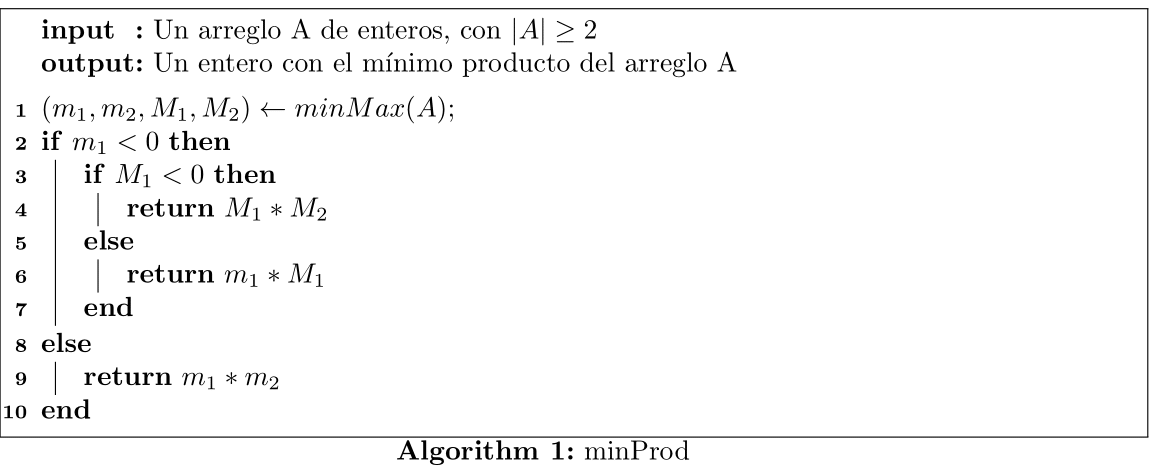
\includegraphics[width=\textwidth]{images/minProd.png}
        \end{figure}
        \begin{figure}[h!]
            \caption{Subrutina que obtiene los valores para minProd}
            \centering
            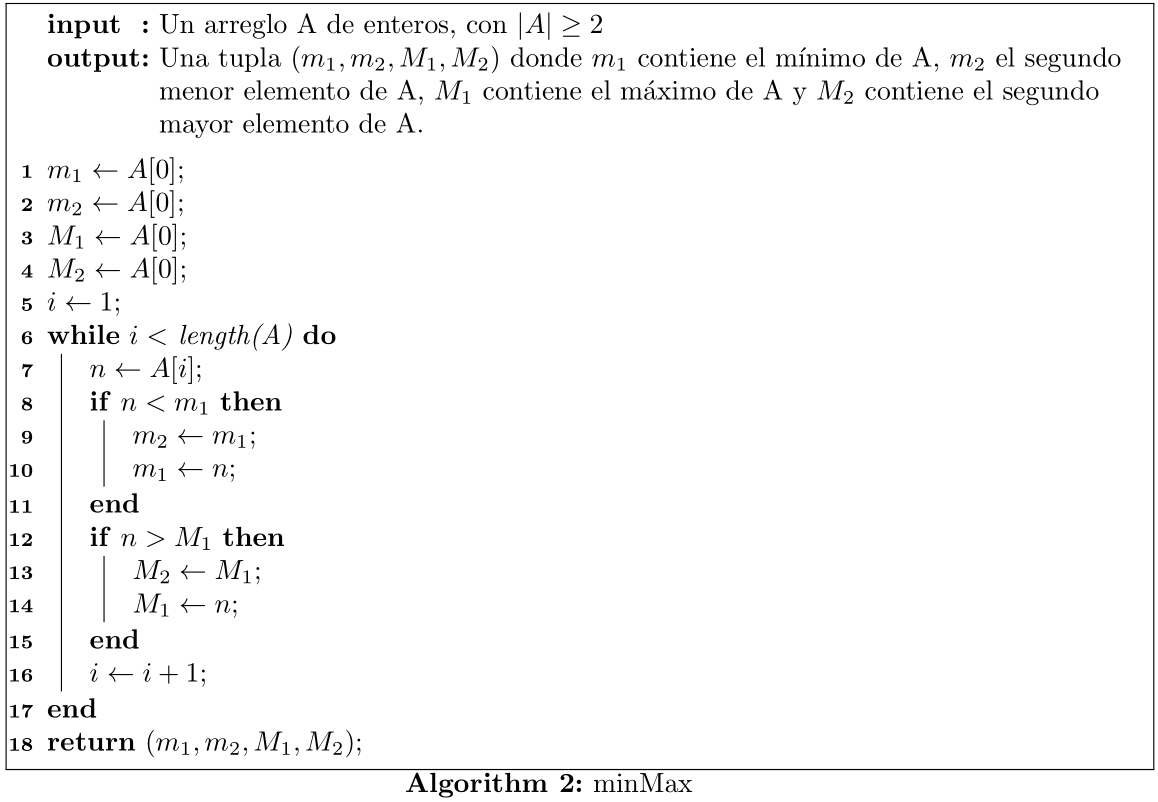
\includegraphics[width=\textwidth]{images/minMax.png}
        \end{figure}


    }
    \item[2)]{}
    \item[3)]{}
\end{enumerate}
}
\end{enumerate}
\end{document}
